\chapter{Verification and Case Studies}

\section{Introduction}
We present a series of numerical simulations to verify and validate our model in this section. Plume-SPH has been verified by comprehensive 1D shock tube tests in previous chapter. In this chapter, it will be further verified by a JPUE (jet or plume that is ejected from a nozzle into a uniform environment) simulation. Velocity and mass fraction distribution both along the central axis and cross transverse are compared with experimental results. The pattern of ambient particles entrainment is also clearly shown. Then a simulation of representative strong volcanic plume, the Pinatubo eruption at June 15th 1991, is conducted. Integrated local variable are comparable with simulation results from existing 3D plume models.

\section{Simulation of JPUE}
JPUE can be considered as a simplified volcanic plume. While the effect of stratified atmosphere and the effect of expansion due to high temperature in volcanic plume are not represented, JPUE reproduces the entrainment due to turbulent mixing which is one of the key elements in volcanic plume development. There exist consistently good experimental data \citep { list1982turbulent,dimotakis1983structure, papanicolaou1988investigations, ezzamel2015dynamical} that describe the JPUE flow field giving an insight into details of JPUE, such as transverse velocity and concentration profile. In this section, we verify that our code and the $SPH-\varepsilon$ turbulence model is able to reproduce feature of turbulent entrainment by a JPUE simulation.

As many of these experiments were conducted with liquid, we replace the original equation of state (Eq. (\ref{eq:EOS})) with a weakly compressible Tait equation of state \citep {becker2007weakly} (see Eq. (\ref{eq:EOS-Tait})) to avoid solving the Poisson equation.
\begin{equation}
p=B\left[\left(\dfrac{\rho}{\rho_0}\right)^{\gamma}-1\right]
\label{eq:EOS-Tait}
\end{equation}
with $\gamma=7$ and $B$ is evaluated by:
\begin{equation}
B=\dfrac{\rho_0 c^2}{\gamma}
\end{equation}
where $c$ is the speed of sound in the liquid. The energy equation is actually decoupled from the momentum conservation equation and the mass conservation equation by using this equation of state (EOS). In addition, the "atmosphere" is assumed to be uniform and gravity is set to be zero. We set the temperature and density of ejected material the same as surrounding ambient. This further simplifies the scenario for the convenience of studying turbulent mixing. 

One overall feature of JPUE is "self-similarity" which means that the evolution of the JPUE is determined solely by the local scale of length and velocity which theoretically account for the fact that the rate of entrainment at the edge of JPUE is proportional to a characteristic velocity at each height. As a results, physical and numerical experiments do not necessary to have exactly the same setups and are compared on a non-dimensional basis.

\begin{table}[htp]
\centering
	\begin{centering}
      \caption{List of eruption condition for the test cases}		
	  \begin{tabular}{lrrr}
	    \hline
	    Parameters & Units  & JPUE & Plume \\
	    \hline
	    Vent velocity          & $m\cdot s^{-1}$  & 500               & 275 \\
	    Vent gas mass fraction &                  & 1.0               & 0.05 \\
	    Vent Temperature       & $K$              & 273               & 1053 \\
	    Vent height            & $m$              & 0                 & 1500 \\
	    Mass discharge rate    & $kg\cdot s^{-1}$ & $5.47 \times 10^7$ & $1.5 \times 10^9$\\
	    \hline
	  \end{tabular}
	  \label{tab:input_parameters}
	\end{centering}
\end{table}

\begin{figure}[!htb]
    \centering
    \begin{minipage}{.425\textwidth}
        \centering
        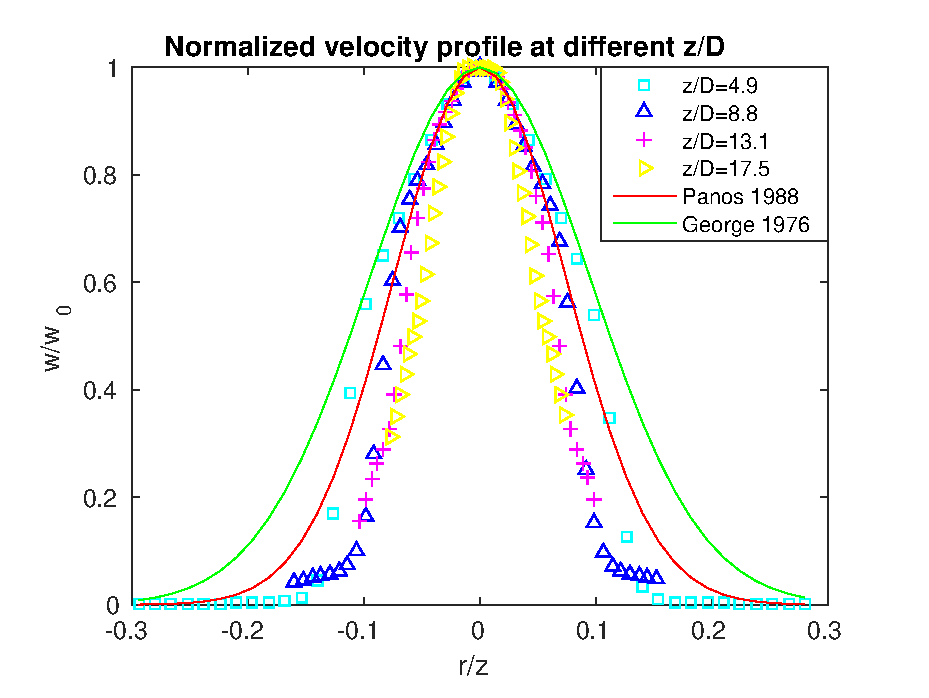
\includegraphics[width=8cm]{Chapter-6/Figures/vel_cross}
    \end{minipage}%
    \begin{minipage}{.425 \textwidth}
        \centering
        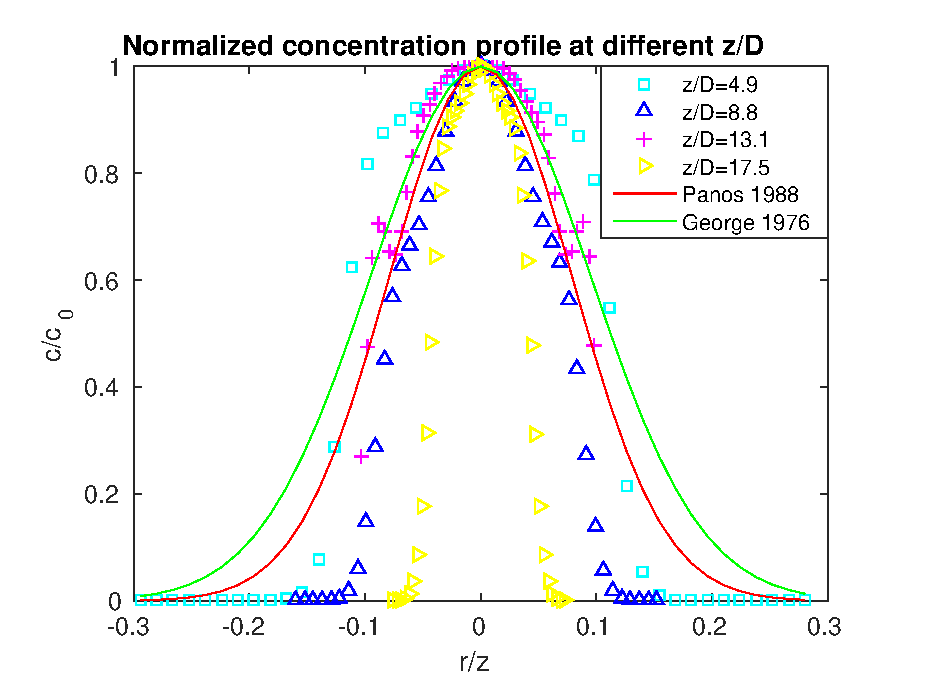
\includegraphics[width=8cm]{Chapter-6/Figures/conc_cross}]
    \end{minipage}%  
    \caption{Dimensionless concentration and velocity distribution across the cross-section.}
    \label{fig:JPUE_cross-section}
\end{figure}

\begin{figure}[!htb]
    \centering
    \begin{minipage}{.425\textwidth}
        \centering
        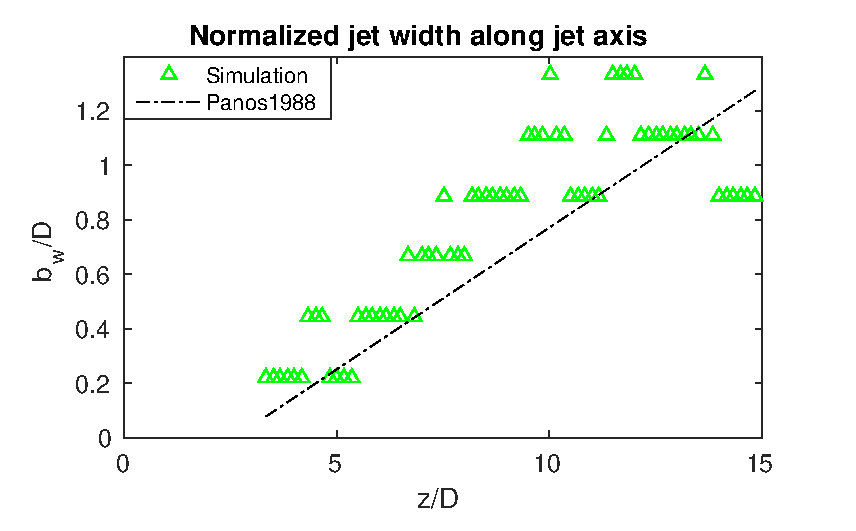
\includegraphics[width=8cm]{Chapter-6/Figures/velo_along_axis}
    \end{minipage}%
    \begin{minipage}{.425 \textwidth}
        \centering
        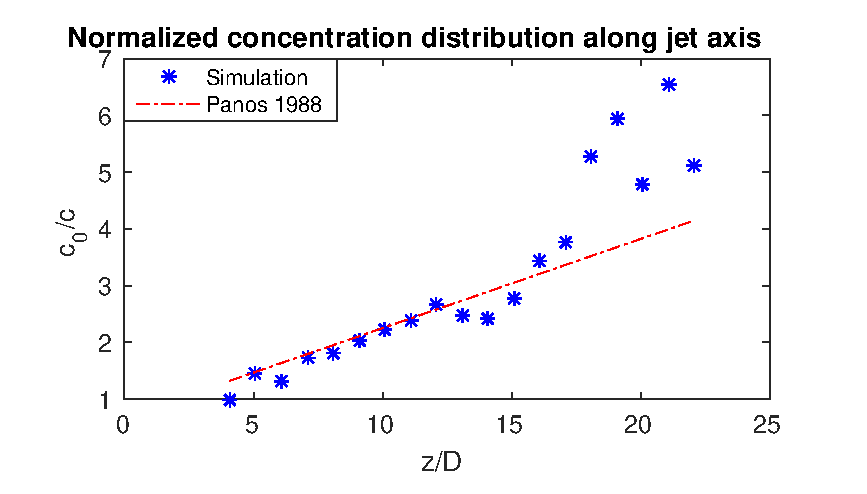
\includegraphics[width=8cm]{Chapter-6/Figures/conc_along_axis}
    \end{minipage}%  
    \caption{The left plot is normalized jet width (which determined based on velocity) along the centerline. The right plot shows normalized concentration along the centerline.}
    \label{fig:JPUE_along-axis}
\end{figure}

A three dimensional axisymmetric JPUE which ejects from a round vent is simulated with eruption parameters listed in Table \ref{tab:input_parameters}. Material properties of water are used as material properties for both phases. The results are compared with experiments \citep {george1977turbulence, papanicolaou1988investigations} for verification purposes. Experimental data of concentration and velocity distribution across the cross-section were fit into a Gaussian profile (See Eq. (\ref{eq:JPUE-experiment-fit-corss})) by \citet{papanicolaou1988investigations} and  \citet{ george1977turbulence} even though the actual profile are slightly different from the Gaussian profile.

\begin{equation}
\dfrac{\varphi}{\varphi_c}=exp \left[-coef\left( \left(\dfrac{r}{z}\right)^2\right)\right]
\label{eq:JPUE-experiment-fit-corss}
\end{equation}

where $\varphi$ is either velocity or concentration, the subscript $c$ represents the centreline. $r$ is the distance from the centreline on any cross-section. $z$ is the axial distance from the origin of the jet transverse section under consideration. 
The coefficient $coef$ for concentration is 80 and 50 respectively according to \citet{george1977turbulence} and \citet{papanicolaou1988investigations}.
$coef$ for velocity is 90 and 55 respectively according to \citet{george1977turbulence} and \citet{papanicolaou1988investigations}. 

\citet{papanicolaou1988investigations} also fit concentration distribution and jet width based on velocity along centerline into a straight line (See Eq. (\ref{eq:JPUE-experiment-fit-along-axis})).. 

\begin{equation}
\dfrac{\varphi_0}{\varphi_c}=slope \left(\dfrac{z}{D} + intercept \right)
\label{eq:JPUE-experiment-fit-along-axis}
\end{equation}

where subscript $0$ represents the cross-sectionally averaged exit value, $D$ is the diameter of vent. 
$slope$ for jet width based on velocity is 0.104 and for concentration is 0.157. 
$intercept$ for jet width based on velocity is 2.58 while that for the concentration is 4.35.

Although both velocity and concentration are found to be well matched with experimental results, a small disparity in both velocity and concentration are observed near the boundary of the jet. Which is possibly caused by overestimating of the drag effect by standard SPH \citep {ritchie2001multiphase}. \citet {ritchie2001multiphase} also proposed an alternative way for density update which releived the overestimating of the drag effect. However, how well does his method conserve mass is not clear. There are several other factors that might also attribute to such disparity. Reynolds number is not reported in many experiments assuming a high enough Reynolds number. In addition, some details of the experiments, such as exit velocity profile and viscosity of the experimental liquid, are not reported. These factors prevent us from numerically reproducing these experiments in an exact way as they were conducted. However, the features of JPUE are correctly reproduced with our code.

We also investigated the mixing due to turbulence in JPUE simulation by checking the mixture of the two phases. It is shown in Fig. \ref{fig:Turb_mixing} that the ejected material and ambient fluids are mixed through eddies at the outer shear region. And the inner dense core dispersed gradually due to erosion of the outer shear region. Hence, our confidence in the numerical correctness of our code is greatly reinforced.

\begin{figure}
\centering
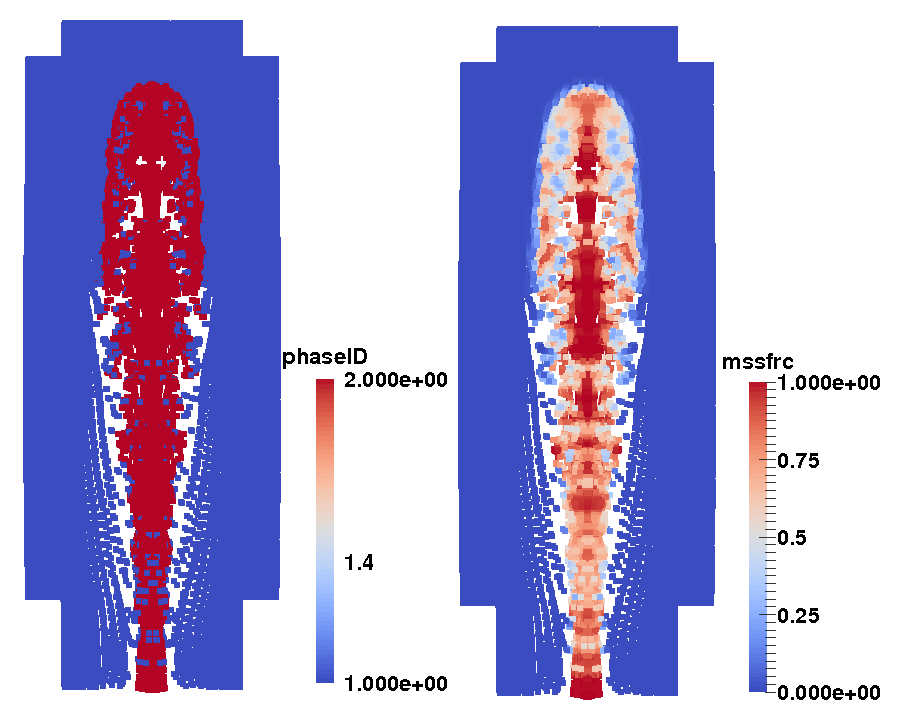
\includegraphics[width=8cm]{Chapter-6/Figures/JPUE_entrainment.png}
\caption{The left figure shows particle distribution. Particles of phase 1 (blue) are gradually entrained and mixed with erupted particles (red) as jet flows down stream. The right figure shows the mass fraction of erupted material at the moment corresponding to the left figure.}
\label{fig:Turb_mixing}
\end{figure}

\section{Simulation of Pinatubo June 15 1991}
The development of a volcanic plume is more complicated than JPUE in several aspects. Besides turbulent entrainment of ambient fluids, development of volcanic plume also involves heating up of entrained air and expanding in a stratified atmosphere. A strong eruption column without wind is tested in this section for the purpose of further verification and validation.
Both global variable and local variables are compared with existing models.

\subsection{Input parameters}
Eruption parameters, material properties and atmosphere are chosen to be the same as the strong plume no wind case in a comparison study on eruptive column models by \citet {costa2016results}. Eruption conditions are listed in Table \ref{tab:input_parameters}. As our model does not distinguish solid particles of different sizes, only mass fraction of solids of all size is used in simulation even though two size classes were provided by \citet {costa2016results}. The density of erupted material at the vent and radius of the vent can be computed from the given parameters. The eruption pressure is assumed to be as the same as pressure of ambient at the vent and hence is not given in the table. The vertical profiles of atmospheric properties were obtained based on the reanalysis data from ECMWF (European Centre for Medium-Range Weather Forecasts) for the period corresponding to the climactic phase of the Pinatubo eruption (Philippines, 15 June 1991). These conditions are more typical of a tropical atmosphere (see Fig. 1B in \citep{costa2016results}). 
%Wind speed is not used in our current model even though it is given (by one component speed from west to east and another component speed from south to north). 
Vertical distribution of temperature, pressure and density is used to establish stratified atmosphere. Wind velocity and specific humidity are not used in our simulation even though they were also provided in Fig. 1B \citep{costa2016results}. Material properties, shown in Table \ref{tab:material_properties}, are selected based on properties of Pinatubo and Shinmoe-dake eruption. Other material properties not given in the table can be inferred from these given parameters based on their relationships.

\begin{table}[htp]
\centering
	\begin{centering}
      \caption{List of material properties}		
	  \begin{tabular}{lrrr}
	    \hline
	    Parameters & Units  & Value \\
	    \hline
	    	Specific heat of gas at constant volume     & $J \cdot kg^{-1}\cdot K^{-1}$& 717     \\
	    Specific heat of air at constant volume     & $J \cdot kg^{-1}\cdot K^{-1}$& 1340    \\
	    	Specific heat of solid                      & $J \cdot kg^{-1}\cdot K^{-1}$& 1100    \\
	    	Specific heat of gas at constant pressure   & $J \cdot kg^{-1}\cdot K^{-1}$& 1000    \\
	    	Specific heat of air at constant pressure   & $J \cdot kg^{-1}\cdot K^{-1}$& 1810    \\
	    	Density of air at vent height               & $kg \cdot m^{-3}$       & 1.104   \\
	    Pressure at vent height                        & $Pa$              & 84363.4 \\
	    \hline
	  \end{tabular}
	  \label{tab:material_properties}
	\end{centering}
\end{table}

Fig. \ref{fig:pinatubo-simulation-results-vis} shows the mass fraction of simulated volcanic plume at 300s after eruption, at which time the plume starts spreading radially. A contour plot of the mass fraction on the vertical cross-section (y-z plane) were also provided. The zoomed view of the quivier plot shows detailed entrainment of air at the margin of the plume.

\begin{figure}[!htb]
    \centering
    \begin{minipage}{.45\textwidth}
        \centering
        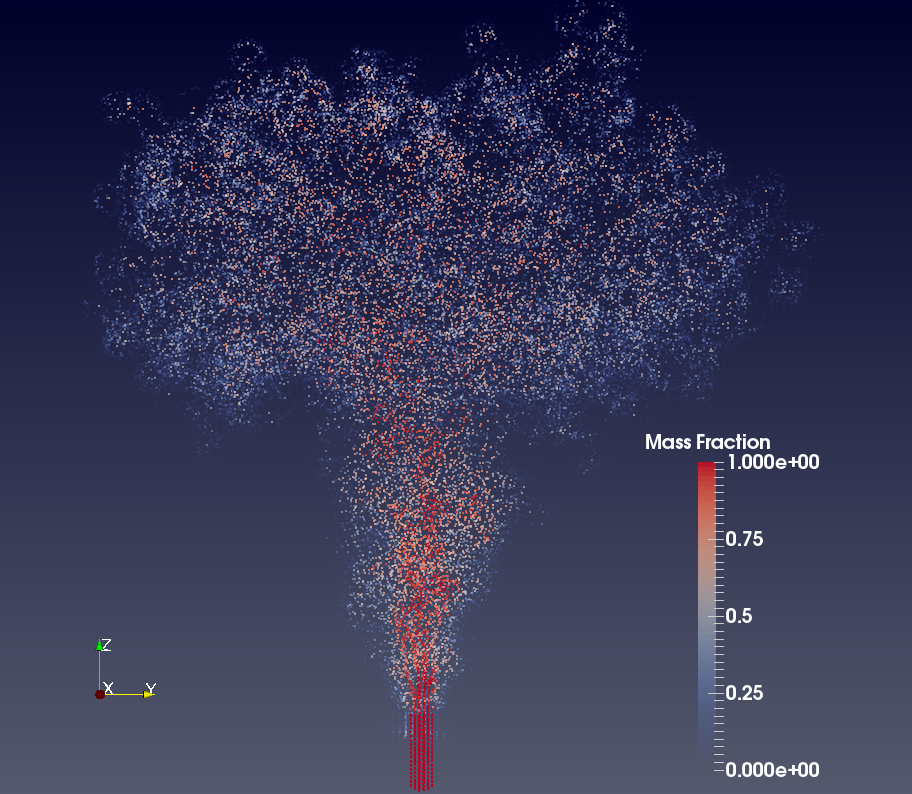
\includegraphics[width=0.99 \textwidth]{Chapter-6/Figures/mssfrc-Diverging}
    \end{minipage}%
    \begin{minipage}{.45 \textwidth}
        \centering
        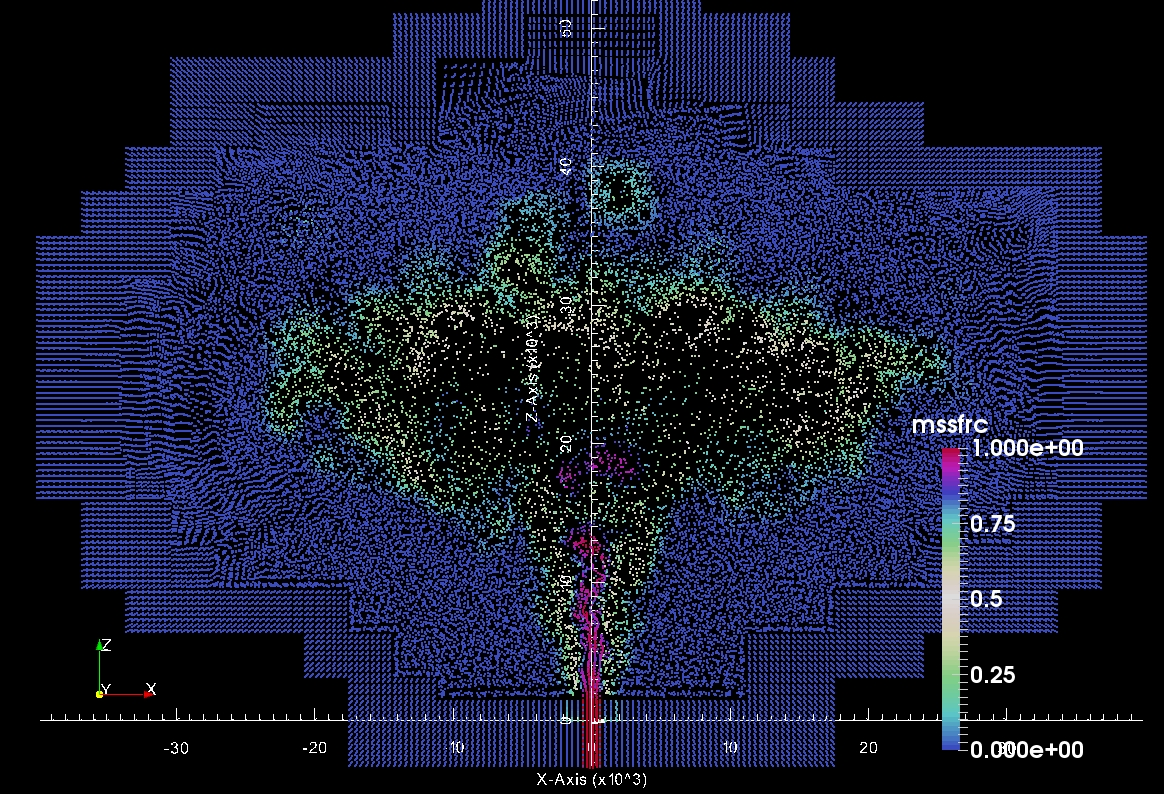
\includegraphics[width=0.99 \textwidth]{Chapter-6/Figures/mssfrc-Diverging-cut}
    \end{minipage}%
    \\
    \begin{minipage}{.45 \textwidth}
        \centering
        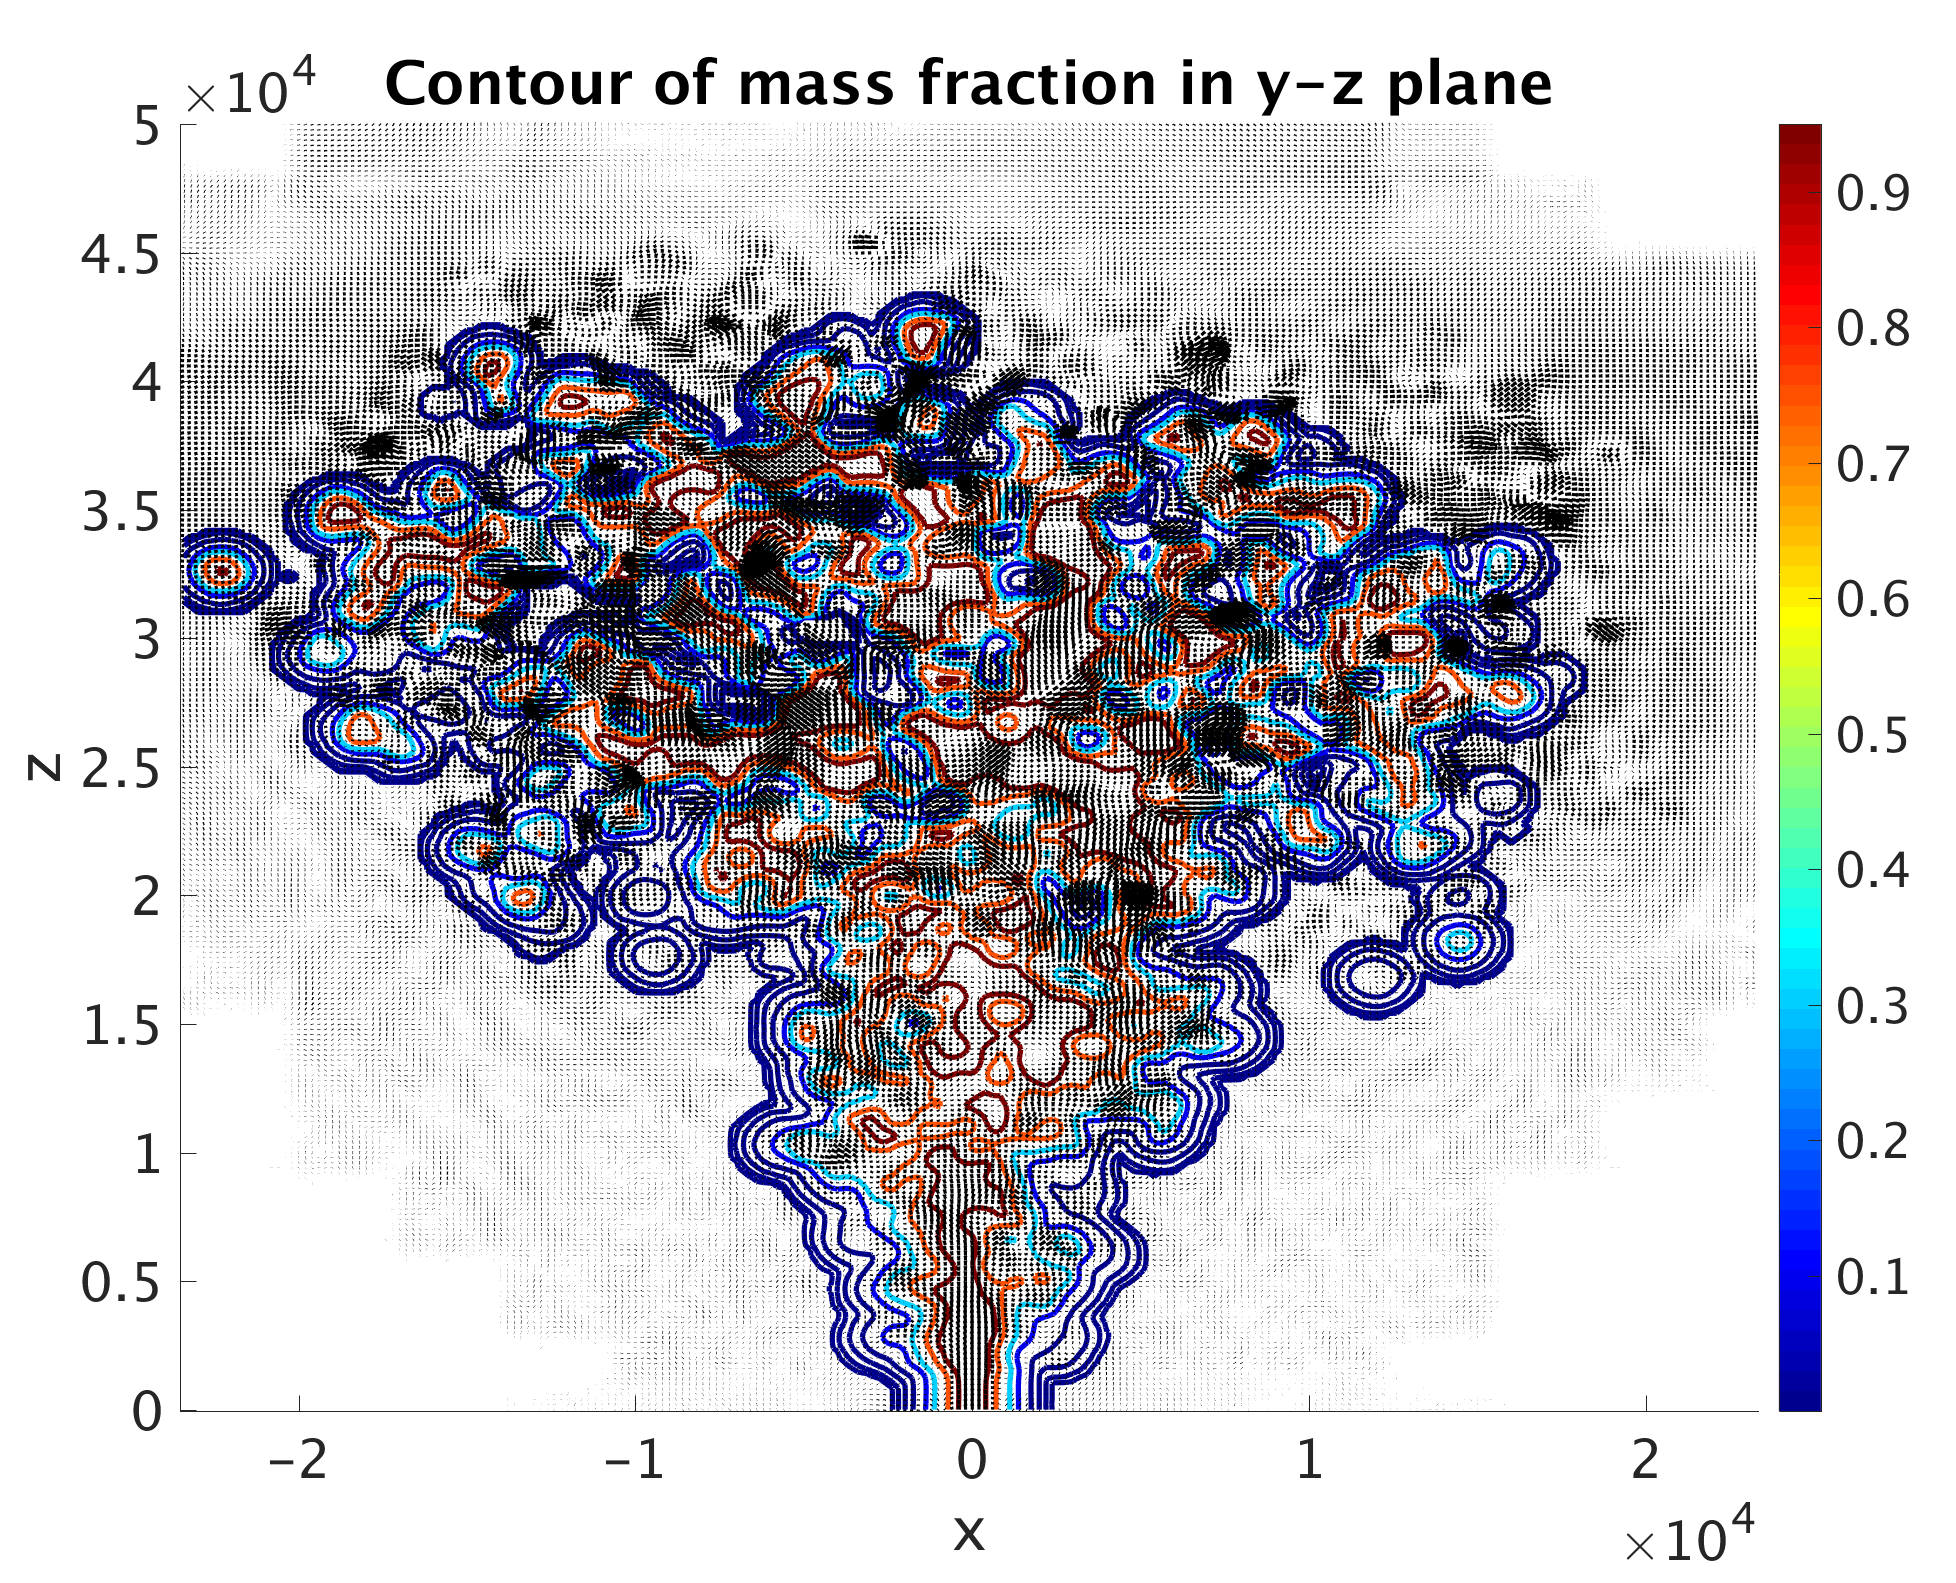
\includegraphics[width=0.99 \textwidth]{Chapter-6/Figures/gmd-mssfrc-yz}
    \end{minipage}% 
    \begin{minipage}{.45 \textwidth}
        \centering
        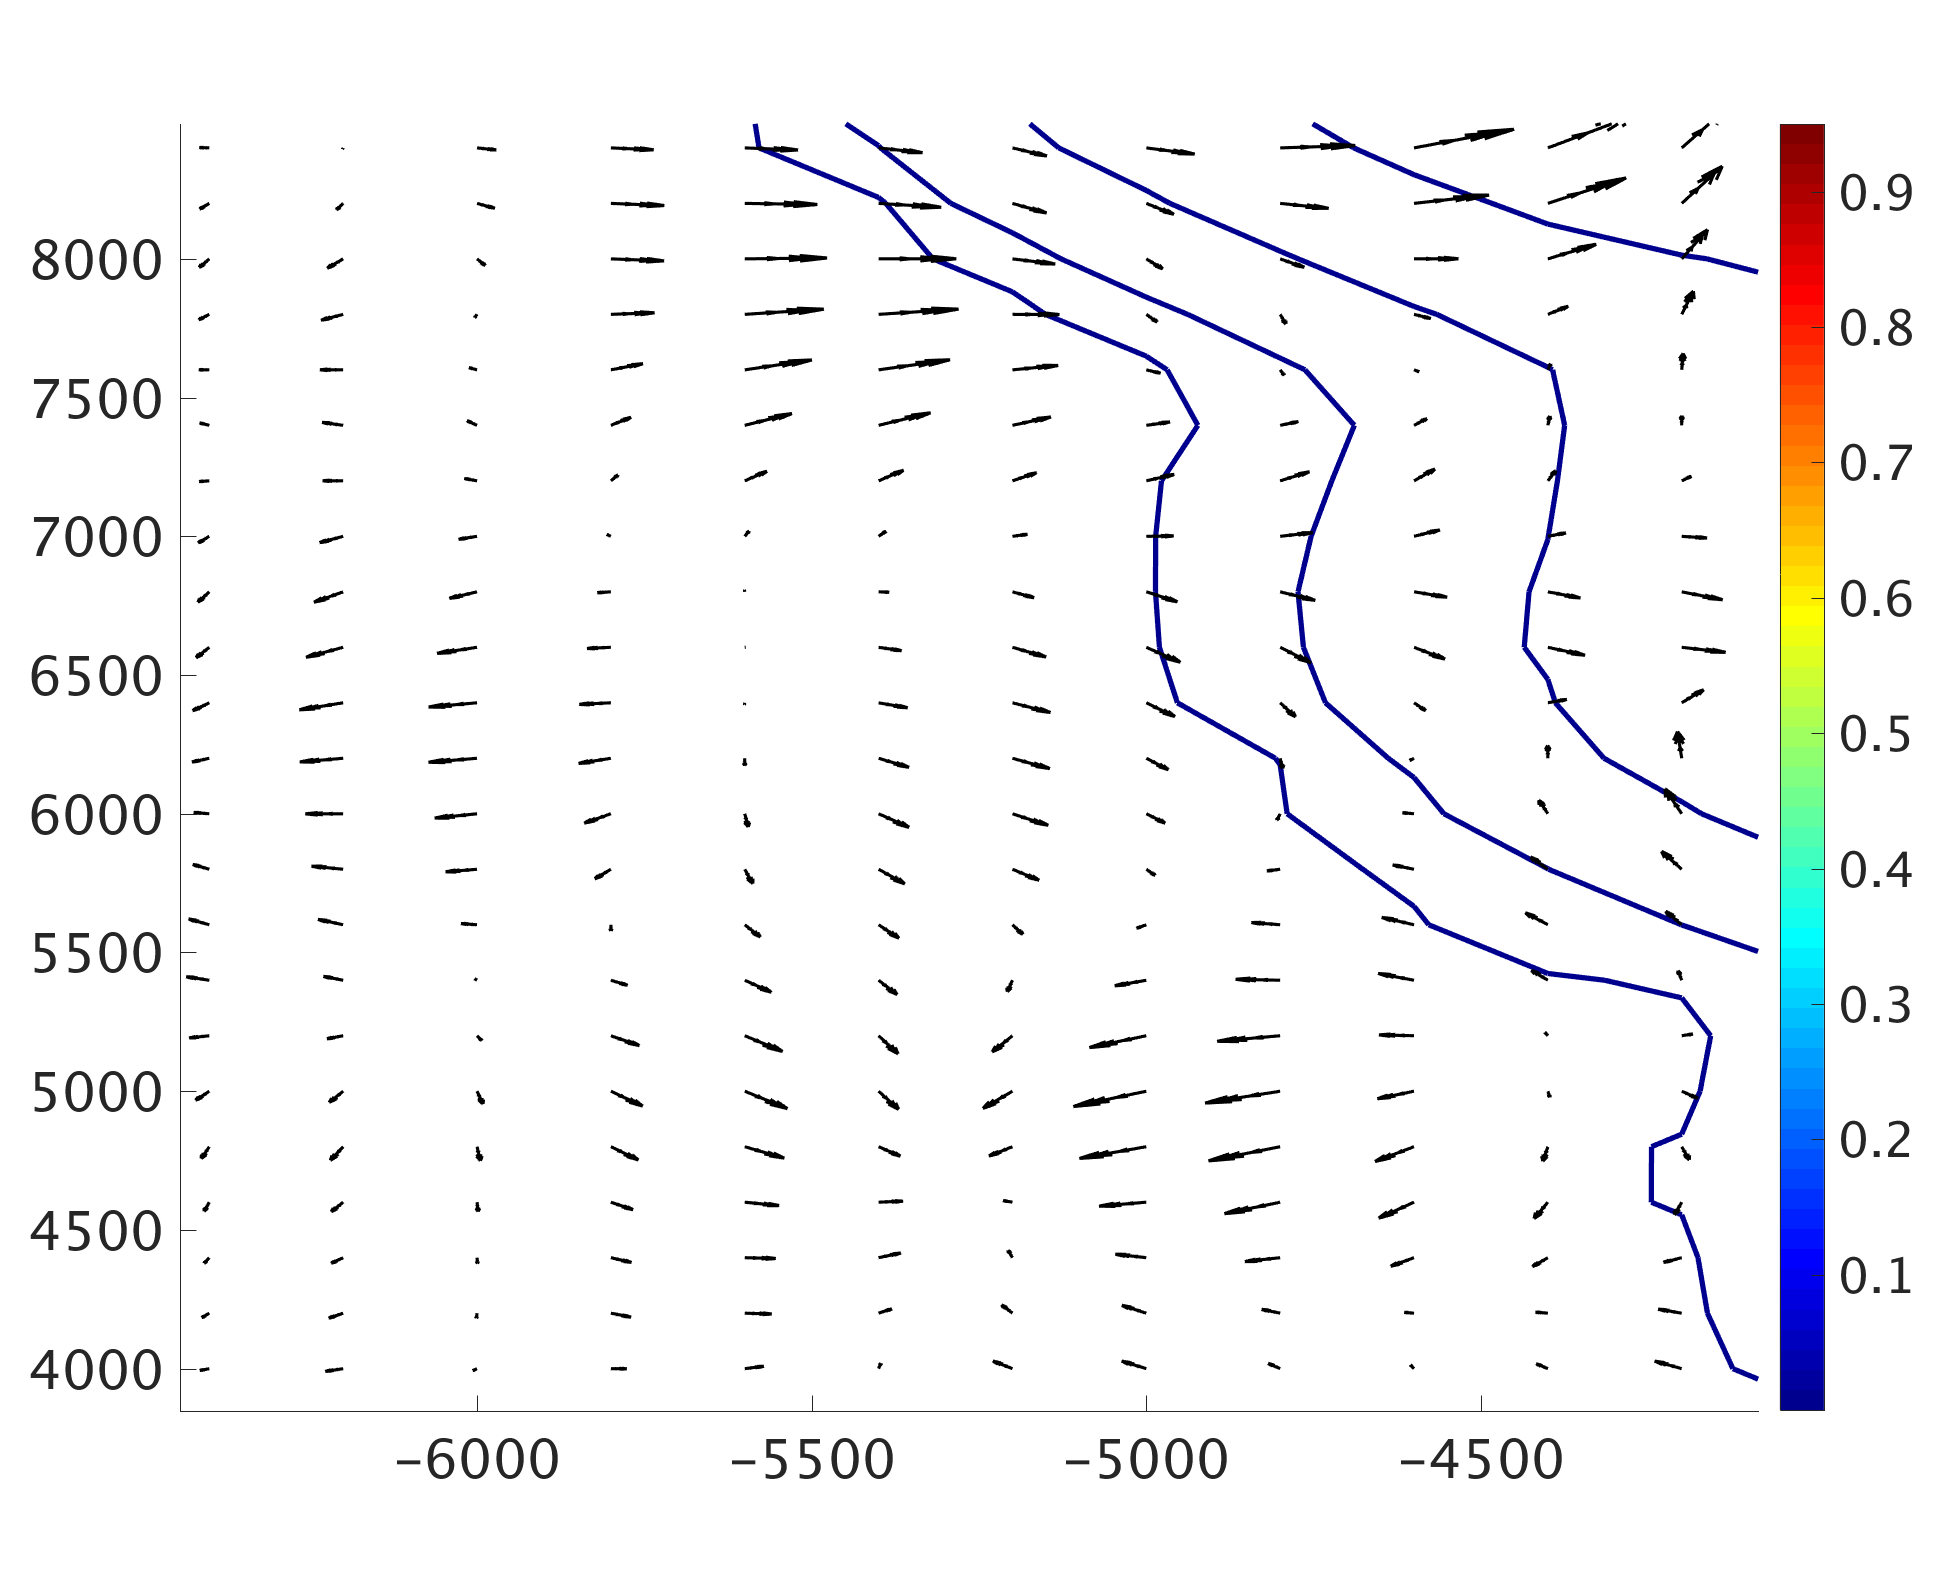
\includegraphics[width=0.99 \textwidth]{Chapter-6/Figures/gmd-mssfrc-yz-zoomed}
    \end{minipage}%  
    \caption{Mass fraction for $t=300s$ after eruption. Figures on the first row are visualization of SPH simulation results. The figure on the up right corner is visualization of a slice of the computational, whose thickness is around $10000m$. The lowest portion of the plume represents erupted material in eruption vent (the underground portition). Figures at the second row show contour of mass fraction and velocity quiver on y-z plane. These figures are plotted utilizing post-processed data (see Appendix \ref{app:project-SPH-grid}). The contour level in the plot are $0.00001, 0.0001, 0.001, 0.1, 0.3, 0.75, 0.95$. The figure on the lower right corner is a zoomed view of velocity quivier showing plume expansion and entrainment of air.}
    \label{fig:pinatubo-simulation-results-vis}
\end{figure}

\subsection{Global and local variables}
One of the key global quantities of great interest is the altitude to which the plume rises. The top height predicted by our model is around 40 km which agrees with other plume models. For example, the height predicted by PDAC is 42500 m, by SK-3D is 39920 m, by ATHAM is 33392 m, by AHSEE is 36700 m. As for local variables, the profiles of integrated temperature, density, mass fraction of entrained air, gas mass fraction, mass fraction of solid and the radius of the plume as a function of height are compared with existing 3D models in Fig. \ref{fig:strong_local_temp} $\sim$ \ref{fig:strong_local_radius}. To get rid of significant fluctuations in time and space we conducted a time averaging and spatial integration of the dynamic 3D flow fields by following \citet {cerminara2016large}.

As particles distribute irregularly in the space in SPH simulation results. We need to project simulation results (on irregular particles) onto a pre-defined grid before doing time average and spatial integration. See appendix A for more details of post processing.

The profiles of local variables match well with simulation results of existing 3D models in a general sense. The basic phenomena in volcanic plume development is correctly captured by our model.

\begin{figure}
\center
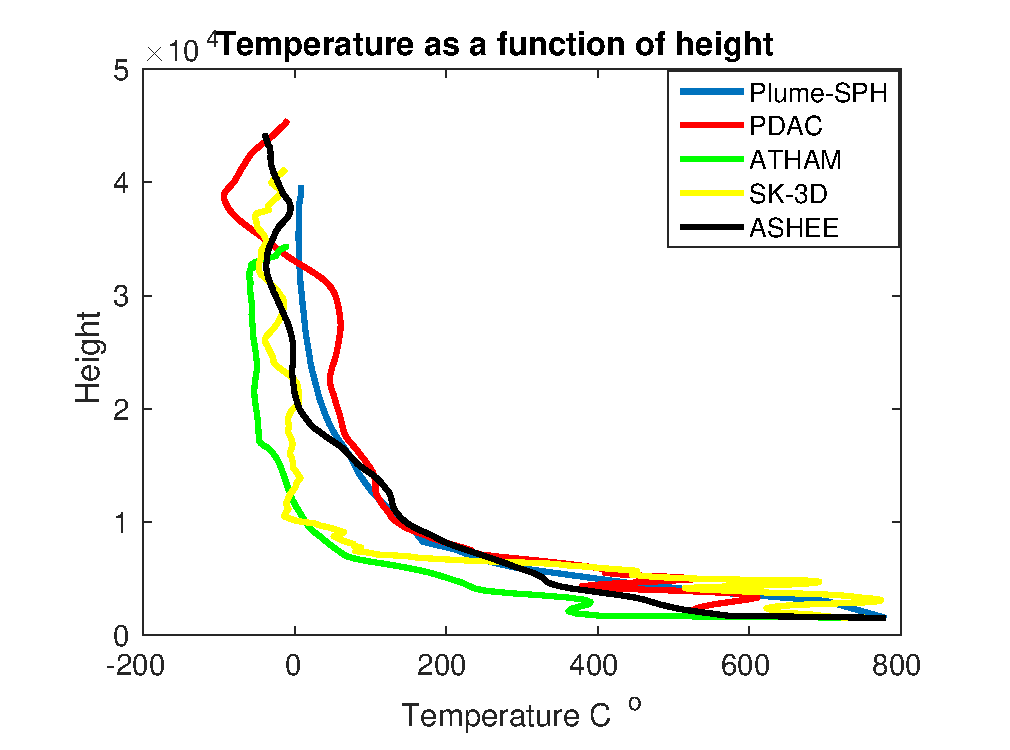
\includegraphics[width=7cm]{Chapter-6/Figures/Temp}
\caption{Temperature as a function of height}
\label{fig:strong_local_temp}
\end{figure}

\begin{figure}
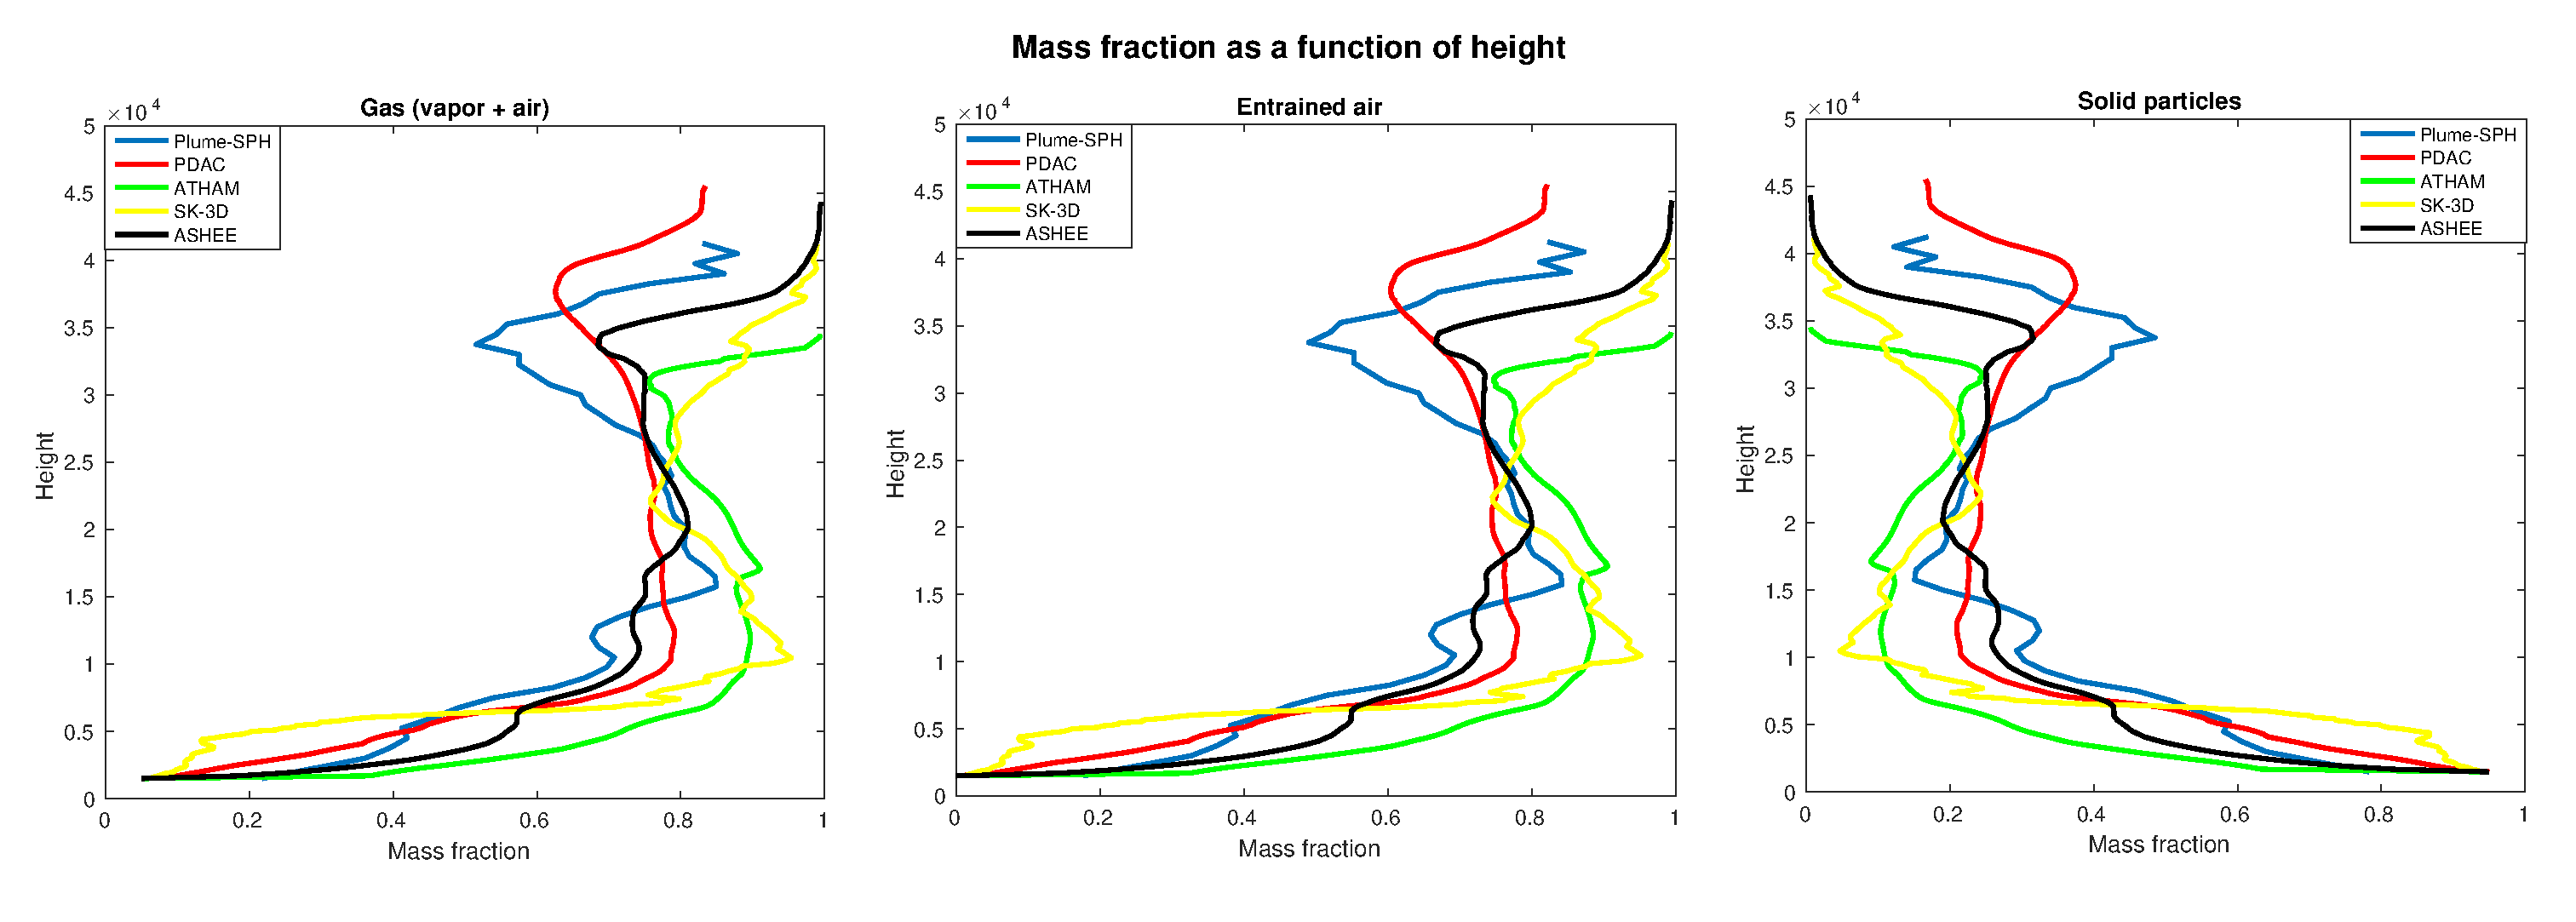
\includegraphics[width=15cm]{Chapter-6/Figures/msfrac}
\caption{The mass fraction of entrained air, gas, and solid as a function of height.}
\label{fig:strong_plume_mass_fraction}
\end{figure}

As the height increases, the amount of entrained air also increases. Around the neutral height, where the umbrella expands, the entrainment of air shows a slight decrease due to lack of air surrounding the column at that height. The profile for gas, which account for both air and vapor, shows a very similar tendency as that of entrained air. Recall that vapor condensation is not considered in our model. In addition, we assume that erupted material behaves like a single phase fluid. So the mass fraction of gas is simply a function of entrained air (Eq. (\ref{eq:gas-frac-express})).
\begin{equation}
\xi_a + \xi_g = \xi_a + \left(1-\xi_a\right) \xi_{g0}
\label{eq:gas-frac-express}
\end{equation}
 
Among these 3D models, ATHAM takes vapor condensation into account and Eq. (\ref{eq:gas-frac-express}) does not hold for ATHAM. However, the profile of entrained air and profile of gas predicted by ATHAM are still very close to each other which implies that ignoring of water phase change is a valid assumption for eruptions similar to this test case (strong plume with erupted water fraction in erupted material less than 5\%). This observation can be explained by the fact that air occupies a larger portion of the gas and ignoring of phase change of vapor (which is only a small portion of gas) causes slight influence on plume development. As for mass fraction of solid, similarly, Eq. (\ref{eq:solid-frac-express1}) and Eq. (\ref{eq:solid-frac-express2}) hold for our model. 
\begin{equation}
\xi_s = \left(1 - \xi_a\right) \left(1- \xi_{g0}\right)
\label{eq:solid-frac-express1}
\end{equation}
\begin{equation}
\xi_s = 1 - \left(\xi_a + \xi_g\right)
\label{eq:solid-frac-express2}
\end{equation}

PDAC, which treats particles of two different sizes as two separate phases, predicted a similar mass fraction profile. That implies that assumption of dynamic equilibrium in our model is at least valid for eruptions similar to the test case.

With more cool air entrained into the plume and mixing with the hot erupted material, the temperature of the plume decreases as the height increases as shown in Fig. \ref{fig:strong_local_temp}. In the meanwhile, bulk density decrease due to entrainment and expansion (Fig. \ref{fig:strong_local_density}).
\begin{figure}
\center
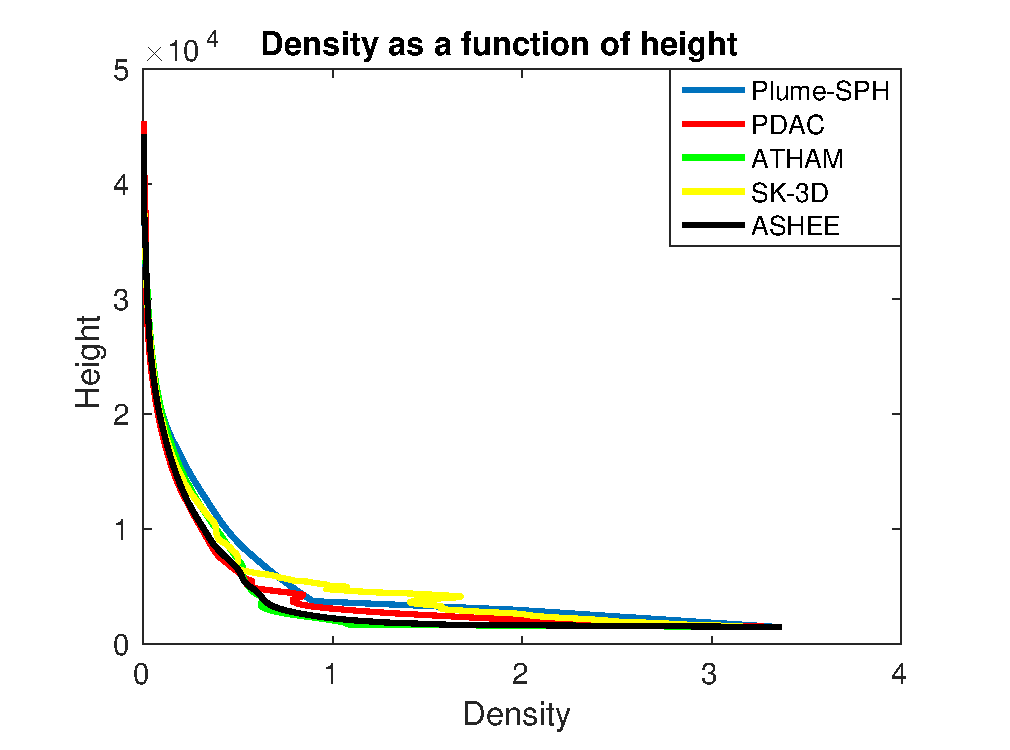
\includegraphics[width=7cm]{Chapter-6/Figures/density_strong}
\caption{Density of the strong plume without wind after reaching its top height}
\label{fig:strong_local_density}
\end{figure}
\begin{figure}
\center
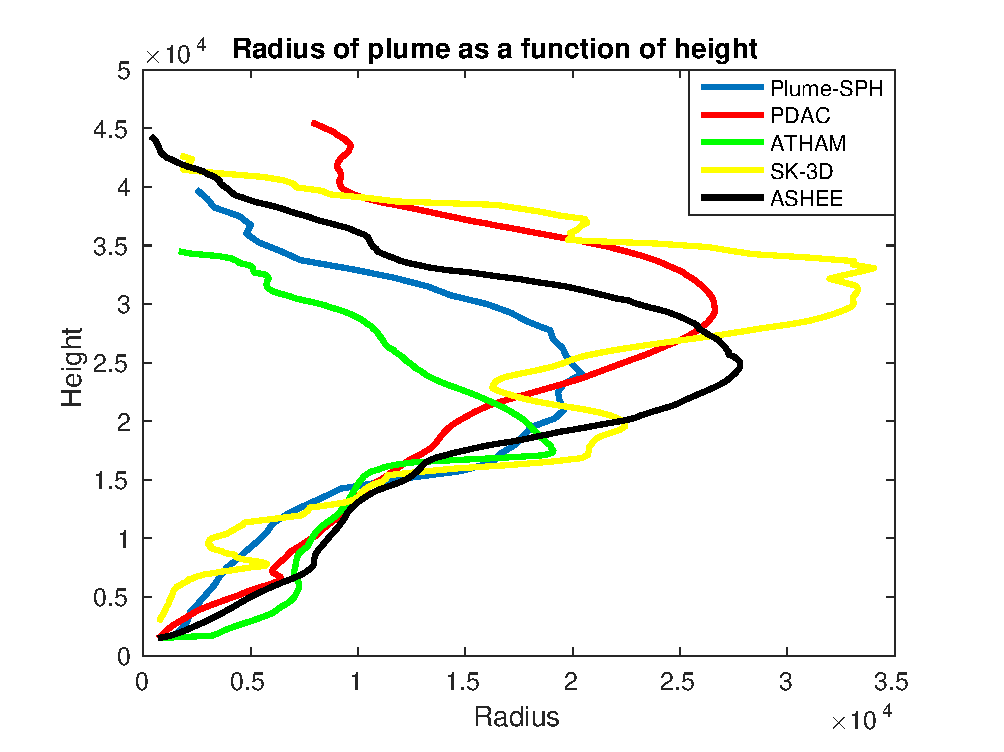
\includegraphics[width=7cm]{Chapter-6/Figures/radius_strong}
\caption{Radius of the strong plume without wind after reaching its top height.}
\label{fig:strong_local_radius}
\end{figure}
Our model adopts the same assumptions and governing equations as SK-3D. However, there is still a obvious disparity between the profiles of local variables of our model and SK-3D. One of the big differences between these two models is that we adopt a LANS type of turbulence model while SK-3D adopts a LES (large eddy simulation) turbulence model. This implies that choice of  turbulence model might play a critical role in plume simulation.

%\subsubsection{Evolution of plume} 
%
%\begin{figure}
%\center
%\includegraphics[width=15cm]{strong_elevation}
%\caption{This figure shows the dynamic evolution process of the Pinatubo with time. At the very beginning, it is driven by initial momentum and rises up quickly, mixing and entraining surround air. Around 100s, the jet stage finishes and it becomes a plume as there were enough air entrained. The plume keeps rising up until reaches the top height then starts spreading.}
%\label{fig:strong_evolution}
%\end{figure}
%
%\begin{figure}
%\includegraphics[width=10cm]{t50}
%\caption{Contour of mass fraction and velocity quiver at 50 seconds in plane x=0, the column keeps rising up and at the same time entraining air into the plume. The zoomed view (right figure) of the quiver plot clearly shows mechanism of air entrainment. The contour levels of mass fraction are 0.7, 0.5, 0.3, 0.1, $1\times 10 ^{-1}$, $1\times 10 ^{-2}$, $1\times 10 ^{-3}$, $1\times 10^{-4}$ and $1\times 10^{-5}$.}
%\label{fig:strong_plume_t50}
%\end{figure}
%
%Figure \ref{fig:strong_evolution} shows the overall evolution process of plume. Plume keeps rising up and entraining air into the plume until it reaches its top height(around t=300 seconds). Afterwards the mixtures of erupted material and air then fall back to neutral height and starts spreading radially. Detailed velocity quiver plot in Fig. \ref{fig:strong_plume_t50} shows entraining of air into the plume at the edge of column. The evolution of the plume further verifies our model.

\section{Conclusion}  \label{sec:conclusion}%% \conclusions[modified heading if necessary]
A new plume model was developed based on the SPH method. Extensions necessary for Lagrangian methodology and compressible flow were made in the formulation of the equations of motion and turbulence models. Advanced numerical techniques in SPH were exploited and tailored for this model. High performance computing was used to mitigate the tradeoff between accuracy (depends on comprehensiveness of the model, resolution, order of accuracy of numerical methods, scheme for time upgrading.) and simulation time (depends on comprehensiveness of model, resolution, order of accuracy of numerical methods, scheme for time upgrading ... and computational techniques). The correctness of the code and model was verified and validated by a series of test simulations. Dimensionless velocity and concentration distribution across the cross-section and along the jet axis match well with experimental results of JPUE. Top height and integrated local variables simulated by our model are consistent with simulation results of existing 3D plume models. Comparison between our results with those of SK-3D implies that turbulence model plays a significant role in plume modeling.

Currently existing 3D models focus on certain aspect of the volcanic plume (PDAC on pyroclastic flow, ATHAM on microphysics, and SK-3D on entrainment with higher accuracy and higher order of accuracy) and hence, naturally, different assumptions were made in these models. However, these different aspects of volcanic plumes are not independent, but are actually coupled. For example, it has been illustrated by \cite{cerminara2016large} that gas-particle non-equilibrium would introduce a previously unrecognized jet-dragging effect, which imposes great influence on plume development, especially for weak plumes. In addition, there is no absolute boundary to determine which kind of hazard is dominant in certain eruptions. So it is necessary to simulate all associated hazards in one model. Actually, effort has already been put on developing more comprehensive plume models. For example, a large-particle module (LPM) was added to ATHAM to track the paths of rocky particles (pyroclastic or tephra) within the plume and predict where these particles fall \citep{kobs2009modeling}. We were also motivated by such an evolution of plume modeling to choose SPH as our numerical tool. Besides its ability in dealing with interfaces for multiphase flows, as mentioned in the introduction section, SPH method has good extensibility and adding new physics and phases requires much less modification of the code compared with mesh based methods. Last but not least, the dramatic development of computational power makes it possible to establish a comprehensive model. While current computational capacity may not allow us to have a fully comprehensive model, the easy-extension feature of SPH makes it convenient to keep adding new physics into the model when necessary and computationally feasible. 

We have presented in this paper an initial effort and results towards developing a first principle based plume model with comprehensive physics, adopting proper numerical tools and high performance computing. More advanced numerical techniques, such as adaptive particle size, Godunov-SPH, semi-explicit time advancing scheme and better data management strategies and algorithms are on our list to exploit in the future. In the near future, effect of wind field will be take into account. Our code will also be made available in the open source form for the community to enhance.
%In all existing 3D plume models, numerical calculations are performed on a non-uniform (vertically and horizontally stretched) grid, with different grid resolutions and domain sizes. However, implementation of different resolution in SPH methods is not straight forward and requires more work.